\documentclass[conference]{IEEEtran}
\IEEEoverridecommandlockouts{}
% The preceding line is only needed to identify funding in the first footnote. If that is unneeded, please comment it out.
%Template version as of 6/27/2024

\usepackage{cite}
\usepackage{amsmath,amssymb,amsfonts}
\usepackage{algorithmic}
\usepackage{graphicx}
\usepackage{textcomp}
\usepackage{xcolor}
\usepackage{hyperref}
\usepackage{cleveref}
\usepackage{lipsum}

\def\BibTeX{{\rm B\kern-.05em{\sc i\kern-.025em b}\kern-.08em
    T\kern-.1667em\lower.7ex\hbox{E}\kern-.125emX}}
\begin{document}

\title{Big Data IU-S25 Assignment 2 Report}

\author{\IEEEauthorblockN{Dmitry Beresnev}
    \IEEEauthorblockA{\textit{Innopolis University} \\
        Innopolis, Russia \\
        d.beresnev@innopolis.university}
}

\maketitle

\begin{abstract}
    It is a report  for the Assignment 2 of Big Data course taught at
    Innopolis University, Russia in Spring semester 2025.
\end{abstract}


\section{Introduction}
A global e-commerce company, faces challenges managing exponential data growth from customer transactions, product catalogs, social networks, and inventory systems. The company wants to find an efficient way to store and analyze the data. They want to see which data model they can use to have fast data retrieval and query processing.

The company is struggling with three big data issues:
\begin{itemize}
    \item \textbf{Volume}: large amounts of data per day
    \item \textbf{Variety}: Social network data, user behavior events, and campaign messages
    \item \textbf{Value}: Analyzing customer social networks for targeted marketing
\end{itemize}

The primary objective of this assignment is to design a big data solution to store petabytes (the provided dataset is only a snapshot) of raw data using effective, optimal and scalable data models that can handle growth and complexity without compromising quality, efficiency, or usability. The optimal design will enable analytics and transactions for real-time and batch data processing. Given task is to find the best data model for storing the big data and obtaining valuable insights from it.

\section{Data Modeling}
You can find the e-commerce dataset description in the assignment description from `reference' directory. Three data models, each for specific database, were designed: Relational (for PostgreSQL), Document (for MongoDB) and Graph (for Neo4j). All the models are designed using Hackolade.

\subsection{Relational Data Model}
The first database version is modeled for PostgreSQL. There are six tables in the relational model, shown in \Cref{fig:postgres_model}: `products', `events', `campaigns', `friends', `clients' and `messages'. This design has the following main features, some of which are inspired by notion of normalization:
\begin{itemize}
    \item Clients are placed in separated table, what removes data redundancy in `message' table. Here i assume that email provider is uniquely defined by client, which lines with dataset description and collected insights
    \item Products with related fields are separated into new table to remove data redundancy in `events' table
    \item In table `campaigns', campaign id ad campaign type are used as primary key, as how is stated in dataset description, campaign id is unique ony within one campaign type. This composite primary key produces corresponding composite foreign key in table `messages', where message type corresponds to campaign type. Once again, this decision does not conflict the dataset description and collected insights, as both types have same set of values
    \item Note, that `event' table, like `products', also has price field. That is because event, like view or purchase, could occur when the price of product was different from the current product price. This feature is also  introduced in other models
\end{itemize}

Other relations, together with data types and foreign and primary keys, shown in \Cref{fig:postgres_model} were deduced from dataset description and are quite natural, so there is no need to describe them in details.

\begin{figure}[htbp]
    \centerline{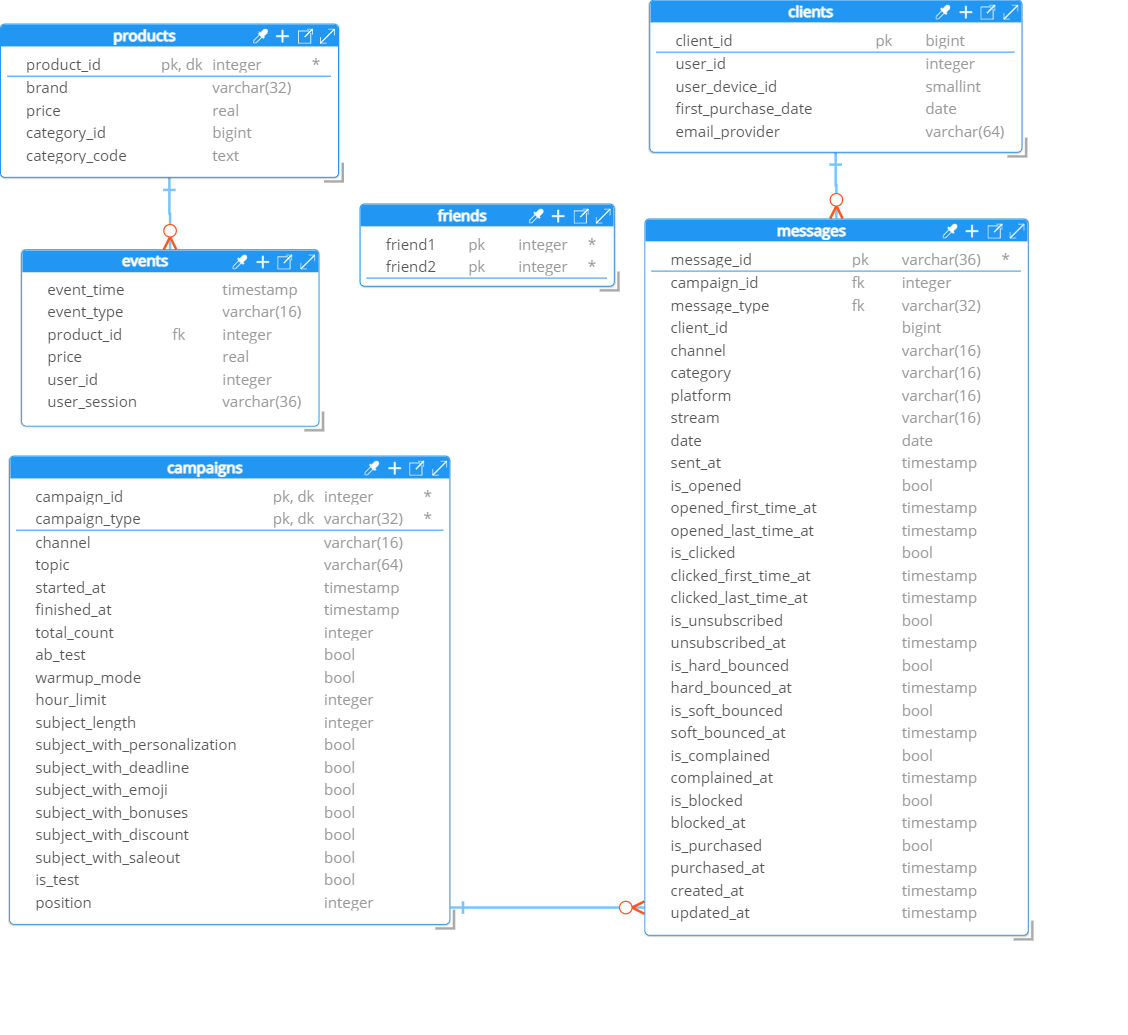
\includegraphics[width=0.5\textwidth]{../screenshots/PostgresModel.png}}
    \caption{Relational Tables for E-commerce}\label{fig:postgres_model}
\end{figure}


\subsection{Document Data Model}
The second database version is modeled for MongoDB.  It creates a unique id by default automatically for each document whenever it is inserted into the database, so there was no need to set special `ObjectID' type to custom identificators.

The main feature of document-based databases is that the data is represented in semi-structured documents: so it is possible to omit some fields if necessary and easily introduce arrays. I have decided to use these feature in the second design. \Cref{fig:mongo_model} shows five collections: `users', `clients', `messages', `campaigns', `products'. Main features of proposed design are the following:
\begin{itemize}
    \item Clients and products are placed in separated tables, as in relational model for same reasons
    \item Document-based model allows to use nested structures, so I decided to combine several fields into sub-documents based on their meaning. For example, fields related to subject within table `campaigns' were combined into field `subject'. Such design produce of more natural and intuitive way of data representation and subsequent querying
    \item Tables `friends' and `events' from relational model were transformed into collection `users', as both tables refers to user id and describe the data related to the specific user: namely his/her friends and events occurred. So the element of collection `users' stores the list of friends and events for specific user
\end{itemize}
Other data types and design elements shown in \Cref{fig:mongo_model} were deduced from dataset description and are quite natural, so there is no need to describe them in details.

\begin{figure}[htbp]
    \centerline{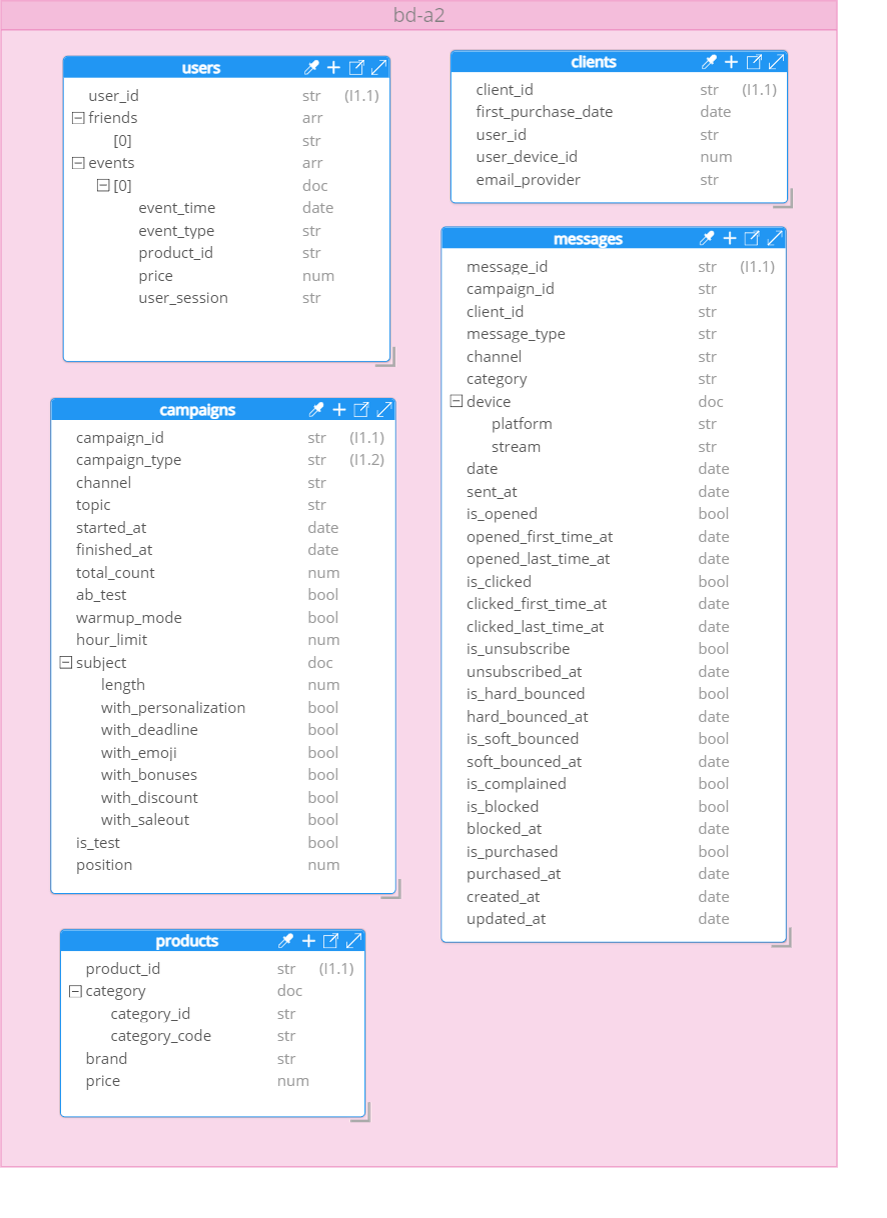
\includegraphics[width=0.45\textwidth]{../screenshots/MongoDBModel.png}}
    \caption{Document Model for E-commerce}\label{fig:mongo_model}
\end{figure}




\subsection{Graph Data Model}
The third database version is modeled for Neo4j.

In a graph model, users and products are represented with nodes, and relationships with edges.
\Cref{fig:neo4j_model} shows the five types of nodes: `Product', `User', `Client', `Message' and `Campaign'. There also are also seven tpe of relationships: `VIEWED', `ADDED TO CART', `PURCHASED' (between user and product), `FRIENDS WITH' (between users), `BELONGS TO' (between client and user), `RECEIVED' (between client and message) and `SENT FROM' (from message to campaign). Properties of nodes and relations are listed in \Cref{fig:neo4j_ermodel}. Main features of proposed design are the following:
\begin{itemize}
    \item Clients and products are placed in separated tables, as in relational and document models for same reasons
    \item Table `events' were transformed to three relationship types: `VIEWED', `ADDED TO CART', `PURCHASED', and the corresponding data transferred to relation properties. The transformation is seemed very natural, as event, in the proposed sense, is indeed a relationships between user and product
    \item Note that the only bi-directional relationship is `FRIENDS WITH', as design of dataset does not imply one-directional friendship. Other relations has naturall hierarchical meaning
\end{itemize}
Other data types and design elements shown in \Cref{fig:neo4j_model,fig:neo4j_ermodel} were deduced from dataset description and are quite natural, so there is no need to describe them in details.

\begin{figure}[htbp]
    \centerline{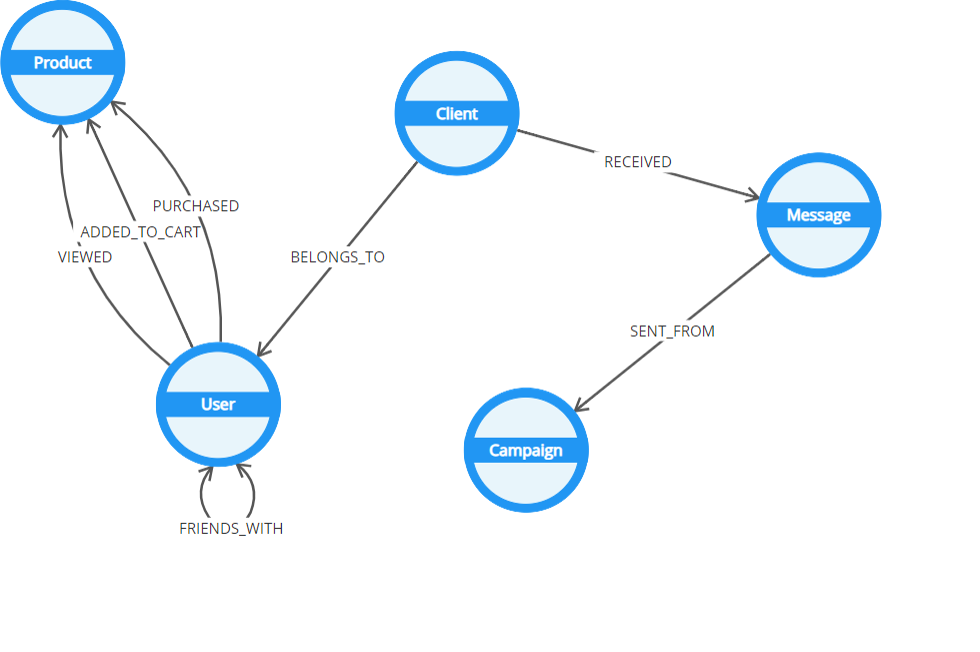
\includegraphics[width=0.4\textwidth]{../screenshots/Neo4jModel.png}}
    \caption{Graph Nodes and Relations for E-commerce}\label{fig:neo4j_model}
\end{figure}

\begin{figure}[htbp]
    \centerline{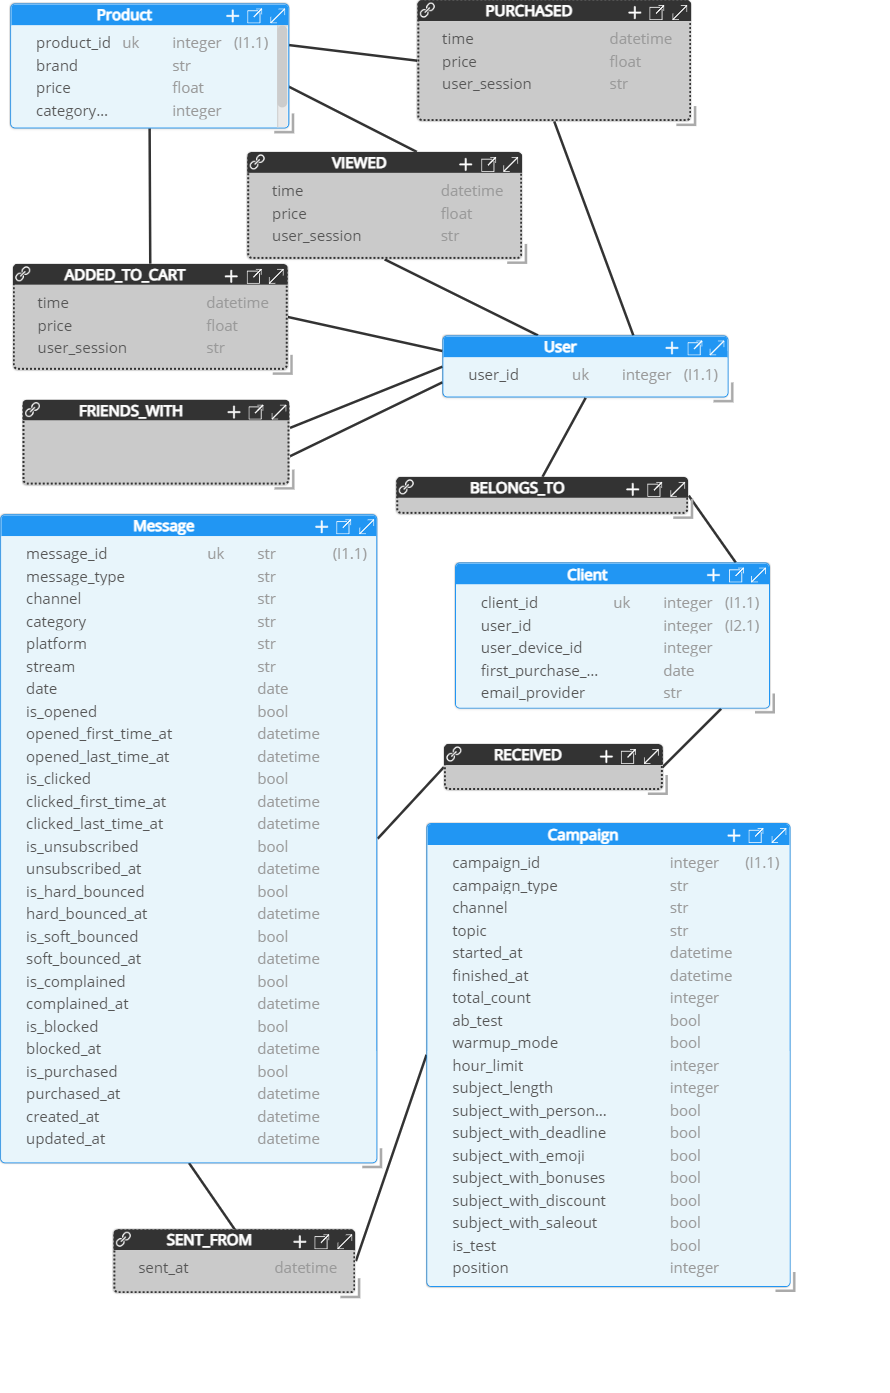
\includegraphics[width=0.5\textwidth]{../screenshots/Neo4jModelER.png}}
    \caption{Graph Model for E-commerce}\label{fig:neo4j_ermodel}
\end{figure}


\subsection{Hybrid Data Model}
The forth approach is to build a hybrid model, which incorporates the advantages of Relational, Document ang Graph models. Proposed hybrid model shown in \Cref{fig:postgres_optimal,fig:mongo_optimal,fig:neo4j_optimal,fig:neo4j_eroptimal} can potentially be better than all models described above. The main characteristics of this approach are the following:
\begin{itemize}
    \item Relational part handles the structured and transactional information, together with transactional relationships, introduced by primary and foreign keys
    \item Document part contains flexible and event-driven data. Fields of this part can be omitted, and new fields can be added on demand. Also, nested documents are introduced for convenient grouping by meaning within items
    \item Graph part effectively handles relationships, the number of which can be enormous. Specifically, it implements friendship, events and user-client relationships.
    \item Note that `event id' is introduced to effectively separate different information about events among Document and Graph parts. For example, Graph part can be used to determine certain event between user and product, and Document part stores information about this event, which can vary depending on event type (though in our case it is the same)
\end{itemize}
Other design features have been already described in corresponding sub-sections, and are mostly natural.

Advantages of hybrid model:
\begin{itemize}
    \item \textbf{Optimization for different purposes}. Relational part can handle transactional data, Document part --- event-driven (and testing) data, and Graph --- relations-related, such as recommendations
    \item \textbf{Scalability and Performance Trade-Off}. Relational part preserves necessary structure, while Document and Graph parts can easily scale horizontally
\end{itemize}

Disadvantages of hybrid model:
\begin{itemize}
    \item \textbf{Complexity}. Maintaining consistency across three databases is complex task
    \item \textbf{Operational overhead}. Expertise in three databases and different types of infrastructures can result in operational inefficiency
    \item \textbf{Slow cross-db communication}. Queries related to multiple databases will usually be slower than in case of one database
\end{itemize}
A
s a result I would recommend using the hybrid model either for small project, where maintaining the consistency is relatively easy, or in quite professional and skill team, which can handle such complex structure.

\begin{figure}[htbp]
    \centerline{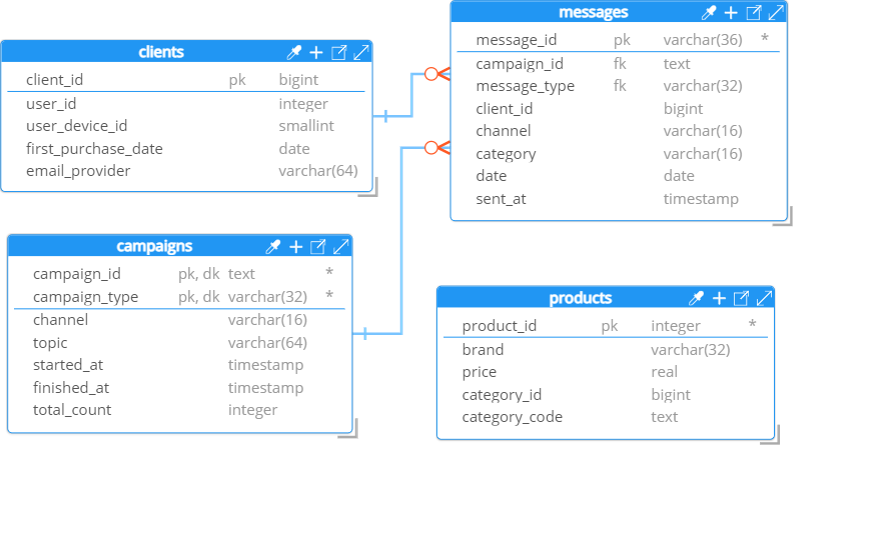
\includegraphics[width=0.45\textwidth]{../screenshots/PostgresModelOptimal.png}}
    \caption{Hybrid Model for E-commerce. Relational part}\label{fig:postgres_optimal}
\end{figure}

\begin{figure}[htbp]
    \centerline{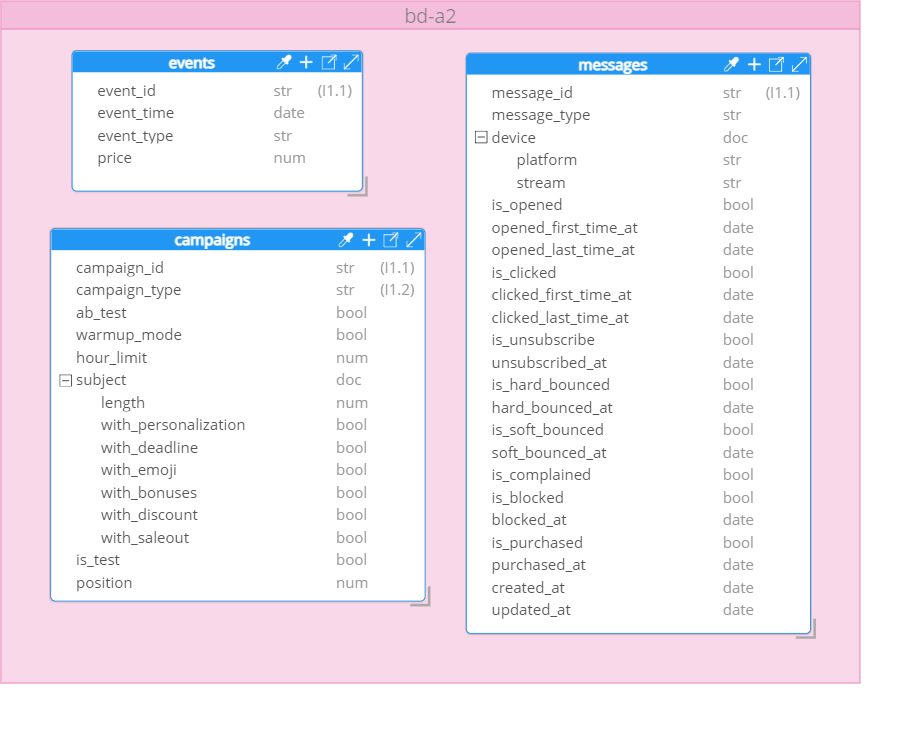
\includegraphics[width=0.45\textwidth]{../screenshots/MongoDBModelOptimal.png}}
    \caption{Hybrid Model for E-commerce. Document part}\label{fig:mongo_optimal}
\end{figure}


\begin{figure}[htbp]
    \centerline{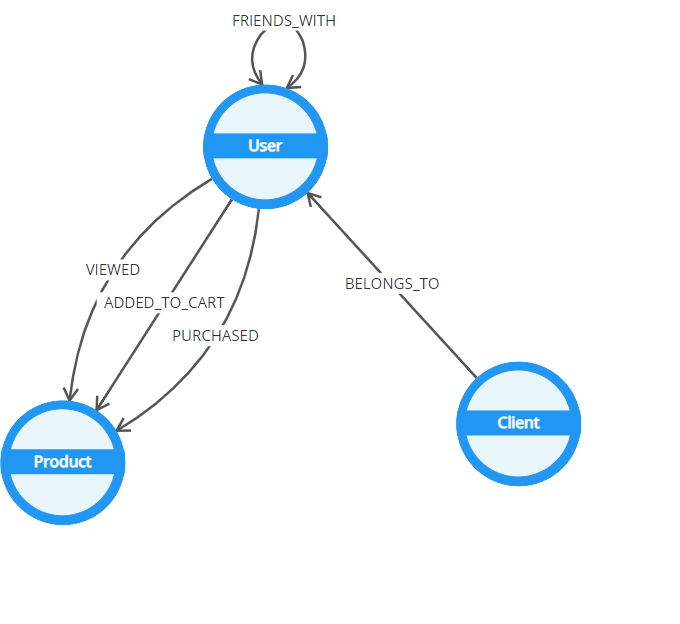
\includegraphics[width=0.3\textwidth]{../screenshots/Neo4jModelOptimal.png}}
    \caption{Hybrid Model for E-commerce. Nodes and relations of Graph part}\label{fig:neo4j_optimal}
\end{figure}

\begin{figure}[htbp]
    \centerline{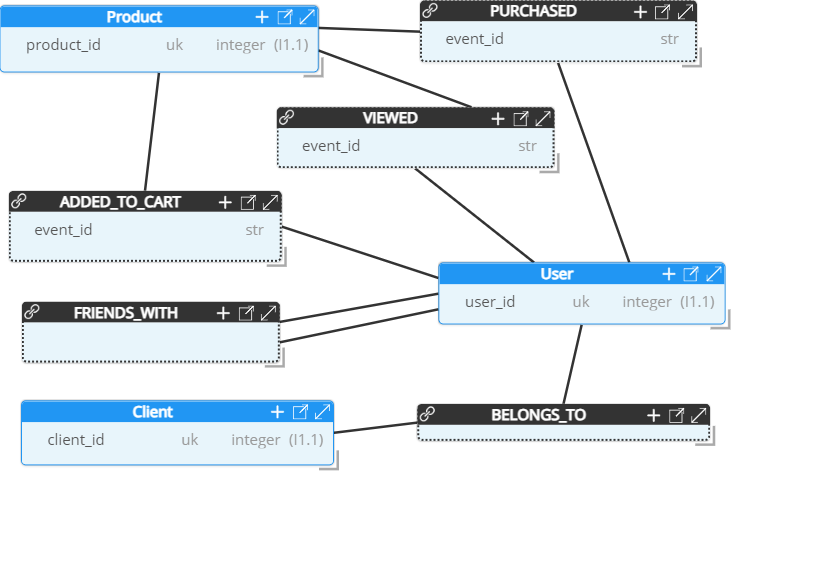
\includegraphics[width=0.5\textwidth]{../screenshots/Neo4jModelEROptimal.png}}
    \caption{Hybrid Model for E-commerce. Graph part}\label{fig:neo4j_eroptimal}
\end{figure}

\section*{Acknowledgment}

The style of this report is inspired by the~\cite{uzunbayir}.


\begin{thebibliography}{00}
    \bibitem{uzunbayir} Serhat Uzunbayir. Relational database and nosql inspections using mongodb and neo4j on a big data application.
    In 2022 7th International Conference on Computer Science and Engineering (UBMK), pages 148--153, 2022.
    doi:10.1109/UBMK55850.2022.9919589.
\end{thebibliography}


\end{document}
